\subsection{Diseño del sistema}

Primero veamos como se comporta el sistema en general. Para eso, utilizaremos un diagrama de clases.

{\color{red} Poner \url{https://www.draw.io/#G0B3FgdUXk8fTrcExpNDN6cl9Manc} cuando esté completo.}

Analicemos y justifiquemos el diagrama parte por parte.

\begin{itemize}
\item[Ubicación] Va a ser la clase que nos va a abstraer de las diferentes posibles representaciones para la ubicación de un bar, en particular el String que representa su dirección, y su latitud y longitud que va a ser útil para calcular distancias, y en general para interactuar con la API de Google Maps, que vamos a usar fuertemente.

\item[Bar] Va a ser la clase que va representar a los bares de la realidad. Los bares tienen una ubicación y una lista de dueños.

\item[PerfilDeBar] Es la clase que nos permite representar un bar desde el punto de vista de la aplicación. Para nuestra aplicación un bar es más que simplemente una dirección y una lista de dueños: un bar tiene votos y comentarios. La clase PerfilDeBar debe pensarse como simplemente un wrapper para la clase Bar, que contiene información pertinente a la aplicación.

\item[ConjuntoDeBares] Representa a todos los bares que existen en la aplicación.Existe porque nos pareció mejor tener una clase separada que abstraiga esta idea, que tener simplemente un conjunto de bares hardcodeado adentro de BuscadorDeBares.

\item[BuscadorDeBares] Es la clase que nos va a permitir buscar bares. Tiene como colaborador interno un ConjuntoDeBares que es el conjunto sobre el cual va a buscar. Recibe un único mensaje que es buscar, que toma como parámetro un filtro.
\end{itemize}


\begin{figure}[H]
  \centering
  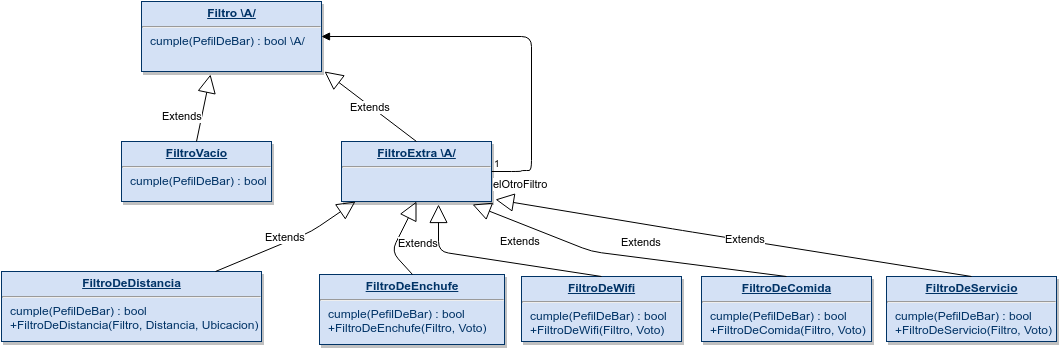
\includegraphics[width=\textwidth]{diagramas/filtro_clases.png}
  \caption{\normalfont Diagrama de clases del subsistema de filtro.}
\end{figure}

\begin{itemize}
\item[Filtro] Para la clase filtro vamos a utilizar el patrón Decorator. Filtro es una clase abstracta, que tiene un mensaje llamado cumple, que recibe un PerfilDeBar y chequea que cumpla su condición. En caso de que la cumpla, va a devolver True, en caso que no, False. Al final del trabajo hablamos más en detalle sobre porqu\'e tomamos las desiciones que tomamos.

\item[FiltroVacio] Va a ser el filtro trivial que nos va a permitir finalizar la composición de filtros, como indica el patron Decorator. Su implementación de cumple va a ser \texttt{return True;}.

\item[FiltroExtra] Va a ser la clase abstracta que nos va a permitir componer filtros. Nótese que tiene como colaborador interno otro Filtro, entonces las clases que hereden de filtro extra, en su implementacion de cumple van a tener que chequear que su condición se cumpla, y que la condición del colaborador interno se cumpla.

\item[FiltroDeX] Van a ser las clases concretas que nos van a permitir filtrar por las diferentes características de un PerfilDeBar. Un comentario importante: la signatura de cumple en nuestra implementación de FiltroDeDistancia difiere un poco de la presentada en el diagrama, pero tiene que ver con temas implementativos de la API de Google Maps que no pudimos evitar; aunque debe tenerse en cuenta que la idea de alto nivel es la misma.
\end{itemize}

\begin{figure}[H]
  \centering
  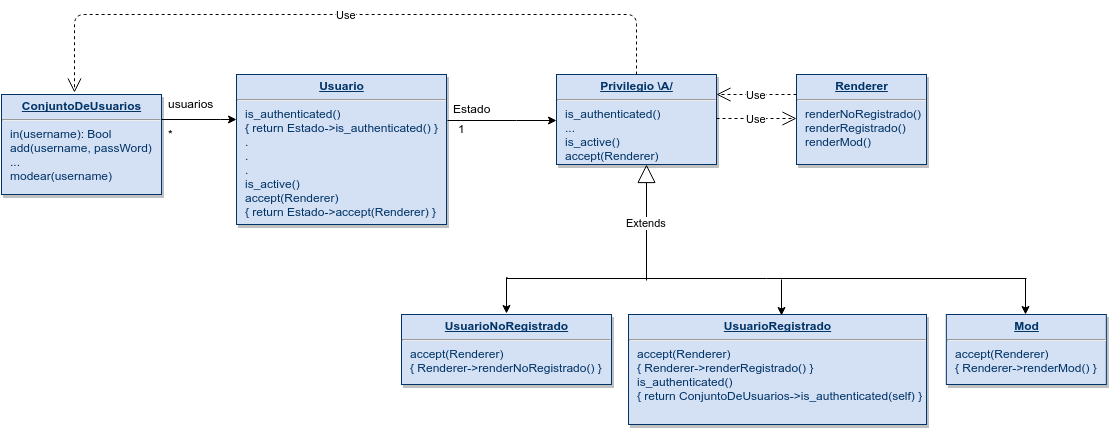
\includegraphics[width=\textwidth]{diagramas/usuario_clases.png}
  \caption{\normalfont Diagrama de clases del subsistema de filtro.}
\end{figure}

\begin{itemize}
\item[ConjuntoDeUsuarios] Como su nombre lo indica, representa el conjunto de usuarios del sistema. Adicionalmente, esta clase es la encargada de validar las credenciales provistas para loguearlos y autenticarlos.
    \par Implementativamente, se accede mediante un \textit{Singleton}.
\item[Usuario] Ésta es la clase que representa a un usuario. 
    Los usuarios pueden tener distintos privilegios\footnote{Actualmente, un usuario puede ser No-Registrado, Registrado o Mod.}, y éstos pueden cambiar en \textit{runtime}; para contemplar esto, empleamos el patrón de diseño \textit{State}\footnote{Empleando la terminología de ``\textit{Design Patterns}'' de Gamma et al, Usuario es el \textit{Context} del patrón.}.
        \par Cabe destacar que la clase usuario presenta ciertos mensajes\footnote{Por ejemplo, \tt{is\_authenticated()}.} que deberían ser responsabilidad de ConjuntoDeUsuarios; éstos deben ser implementados por la clase Usuario para poder emplear el módulo \textit{Flask-Login}.
        Nuestros métodos forwardean dichos mensajes a ConjuntoDeUsuarios, ya que son su responsabilidad.
    \item[Privilegio] Como mencionamos, la clase Usuario emplea el patrón \textit{State}; Privilegio es la clase abstracta de la cual heredan los privilegios concretos. En términos de ``\textit{Design Patterns}, Privilegio es el \textit{State} del patrón.
    \item[Mod, etc...] Éstos son los privilegios concretos que puede adquirir un Usuario; son los \textit{Concrete States} del patrón. Como tales, los métodos de Usuario simplemente forwardean los mensajes a estas clases, que se ocupan de realizar la implementación propriamente dicha.
    \item[Renderer] El rendering de HTML al cargar una página\footnote{Podría haber más eventos con requerimientos similares; actualmente el rendering de HTML es el único que se nos presentó, por lo que nos concentraremos en éste. Sin embargo, lo siguiente es aplicable a cualquiera de éstos.} puede depender de los privilegios del usuario actual, pero no es responsabilidad del Usuario.
        \par Para resolver esto, empleamos un patrón \textit{Visitor}: Usuario presenta un mensaje \textit{accept}, cuyo método forwardea el mensaje a Privilegio, y cada privilegio concreto llama al mensaje correspondiente del Renderer\footnote{Que corresponde al \textit{visitor} del patrón, en términos de ``\textit{Design Patterns}''.}.
    \par Cabe destacar que empleamos un único \textit{visitor} concreto, en vez de una jerarquía de \textit{visitors} concretos que heredan de uno abstracto, pues requerimos uno solo. Sin embargo, dado el \textit{duck typing} de \textit{Python}, es trivial refactorear nuestra implementación a una con dicha jerarquía, en caso de requerirlo en el futuro.
\end{itemize}



{\color{red}
\begin{itemize}
  \item[\footnotesize{VisualizadorDeResultados}] asd asd
\end{itemize}
}


\subsection{Diagramas de Objetos y Secuencia}

\subsubsection{Calificar bares}

\subsubsection{Filtro de bares filtrando por una única característica}


\begin{figure}[H]
  \centering
  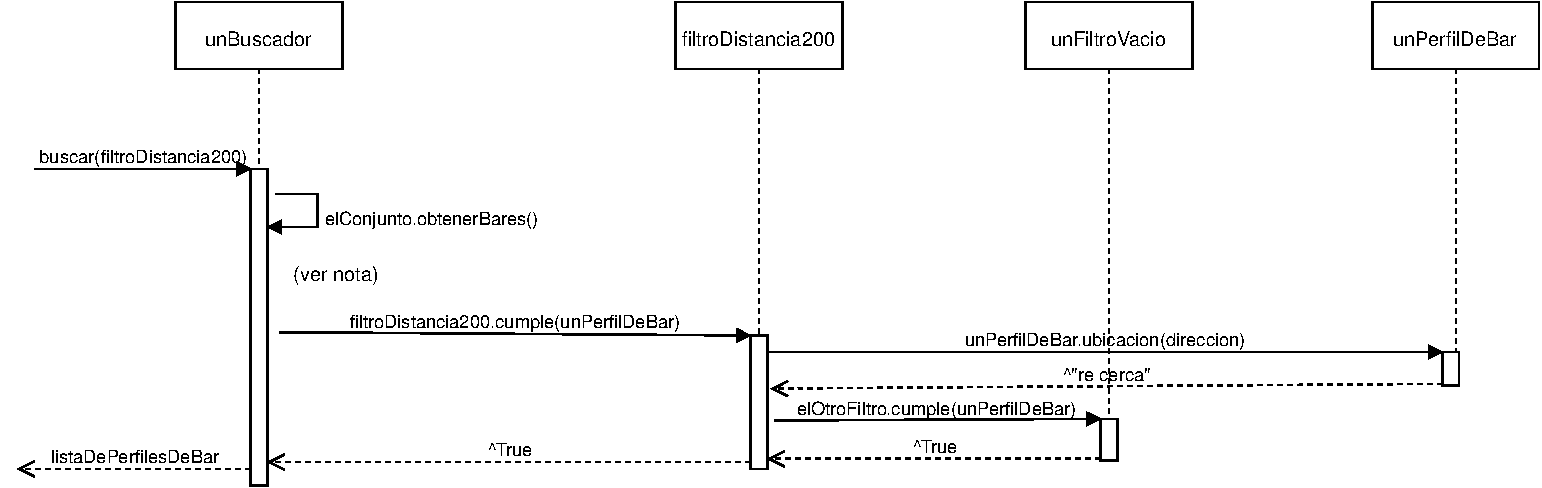
\includegraphics[width=\textwidth]{diagramas/secuencia_2.pdf}
  \caption{\normalfont Diagrama de secuencia. Nota: corremos, \texttt{filter(bares, filtroDist200.cumple)}, por simplicidad ponemos sólo una llamada a cumple.
Además, donde dice "votos", debería decir "valoracionPorcentualPorFeature", pero lo escribimos así para hacerlo más corto y que el diagrama no quede mal.
	}
\end{figure}

\begin{figure}[H]
  \centering
  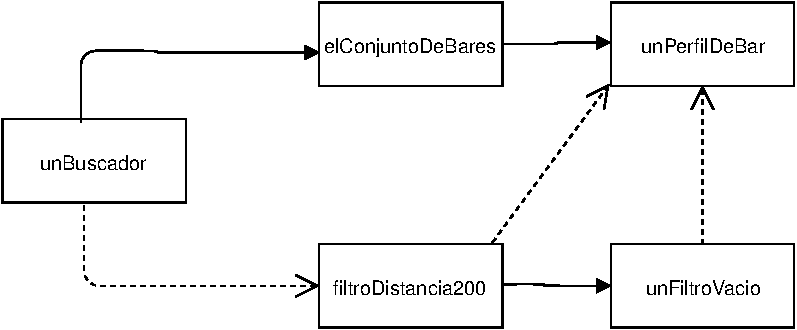
\includegraphics[width=0.7\textwidth]{diagramas/objetos_2.pdf}
  \caption{\normalfont Diagrama de objetos.}
\end{figure}

Cómo se ve claramente, el filtro es un típico ejemplo de uso de Decorator. Como se ve, unBuscador recibe un conjunto de perfiles de bares. Como aclaramos en la nota, lo que hacemos es simplemente llamar a \texttt{filter}, pero ejemplificamos lo que sucede con un perfil específico. En este caso, la distancia del bar es menor que 200, entonces devuelve True.

\subsubsection{Filtro de bares filtrando por tres característica}

\begin{figure}[H]
  \centering
  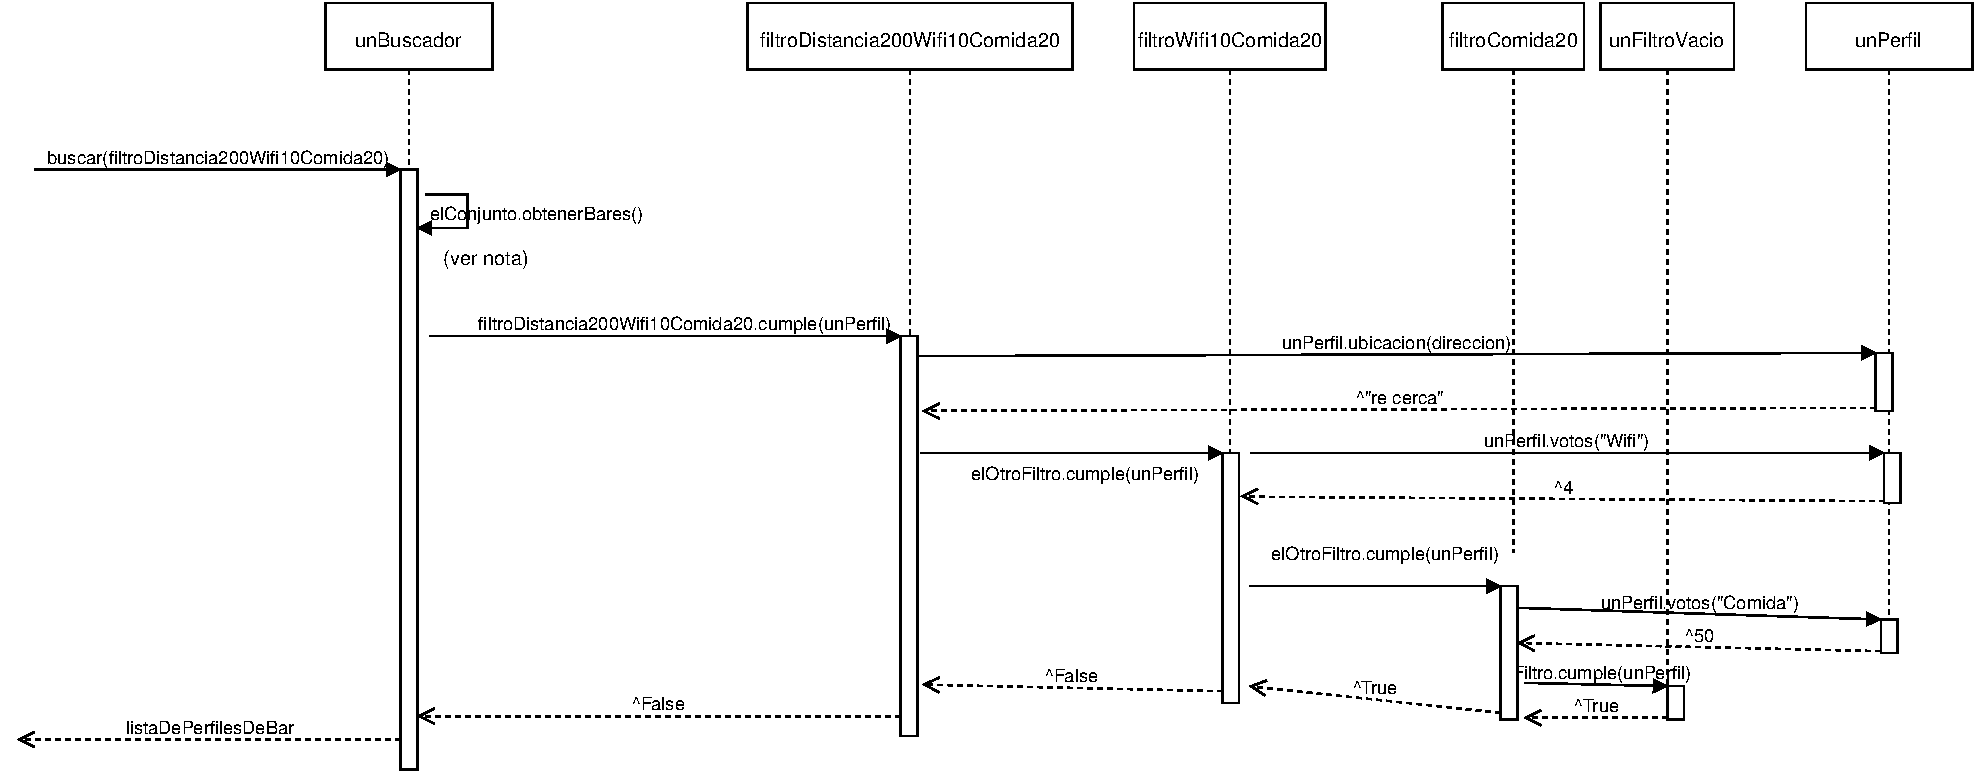
\includegraphics[width=\textwidth]{diagramas/secuencia_3.pdf}
  \caption{\normalfont Nota: \texttt{corremos filter(bares, filtroDist200Wifi10Comida20.cumple)}, por simplicidad ponemos sólo una llamada a cumple.
Además, donde dice "votos", debería decir "valoracionPorcentualPorFeature", pero lo escribimos así para hacerlo más corto y que el diagrama no quede mal.
}
\end{figure}


\begin{figure}[H]
  \centering
  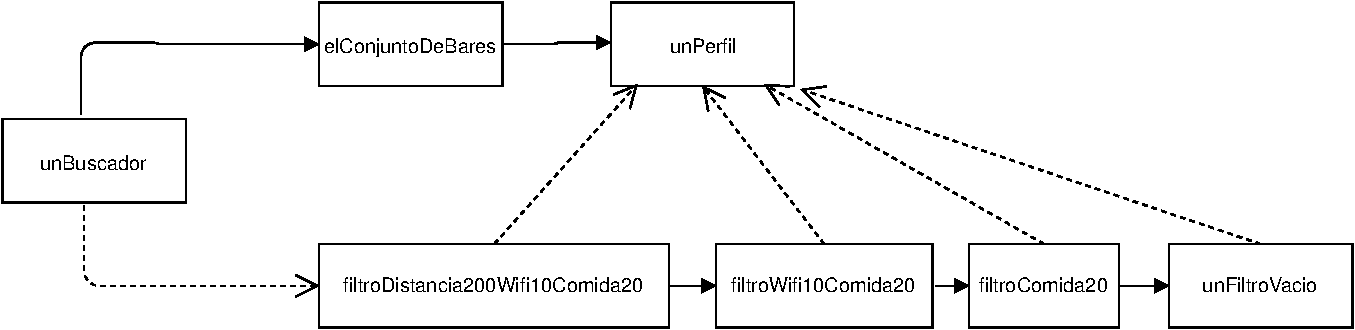
\includegraphics[width=\textwidth]{diagramas/objetos_3.pdf}
  \caption{\normalfont Diagrama de objetos.}
\end{figure}


Igual que arriba, se ve que es un típico ejemplo de uso de Decorator.

Como aclaramos en la nota, lo que hacemos es simplemente llamar a \texttt{filter}, pero ejemplificamos lo que sucede con un perfil específico. En este caso, la distancia al bar es menor que 200, pero la valoración del Wifi es 4, que es menor que 10, con lo cual esa llamada va a devolver False, valor que se va a propagar hacia atrás.

En cuanto al diagrama de objetos es igual que antes. El buscador tiene adentro al conjunto de bares que a su vez tiene adentro a unPerfil. Sin embargo, los filtros solo conocen a los perfiles que le llegan como parámetro.

\subsubsection{Visualización de resultados}

Ahora pasaremos a ver la parte de visualización de resultados. Esta parte fue modelada con una clase llamada VisualizadorDeResultados, que permite encapsular la parte de generación de resultados. En los diagramas no mostramos la parte ``implementativa'' que es la que se ocupa de llamar a Flask para generar el HTML porque creemos que no suma.

Sin embargo, mostramos la parte más vital, que es la de creación de filtro y de búsqueda de resultados. Veamos como es.

\begin{figure}[H]
  \centering
  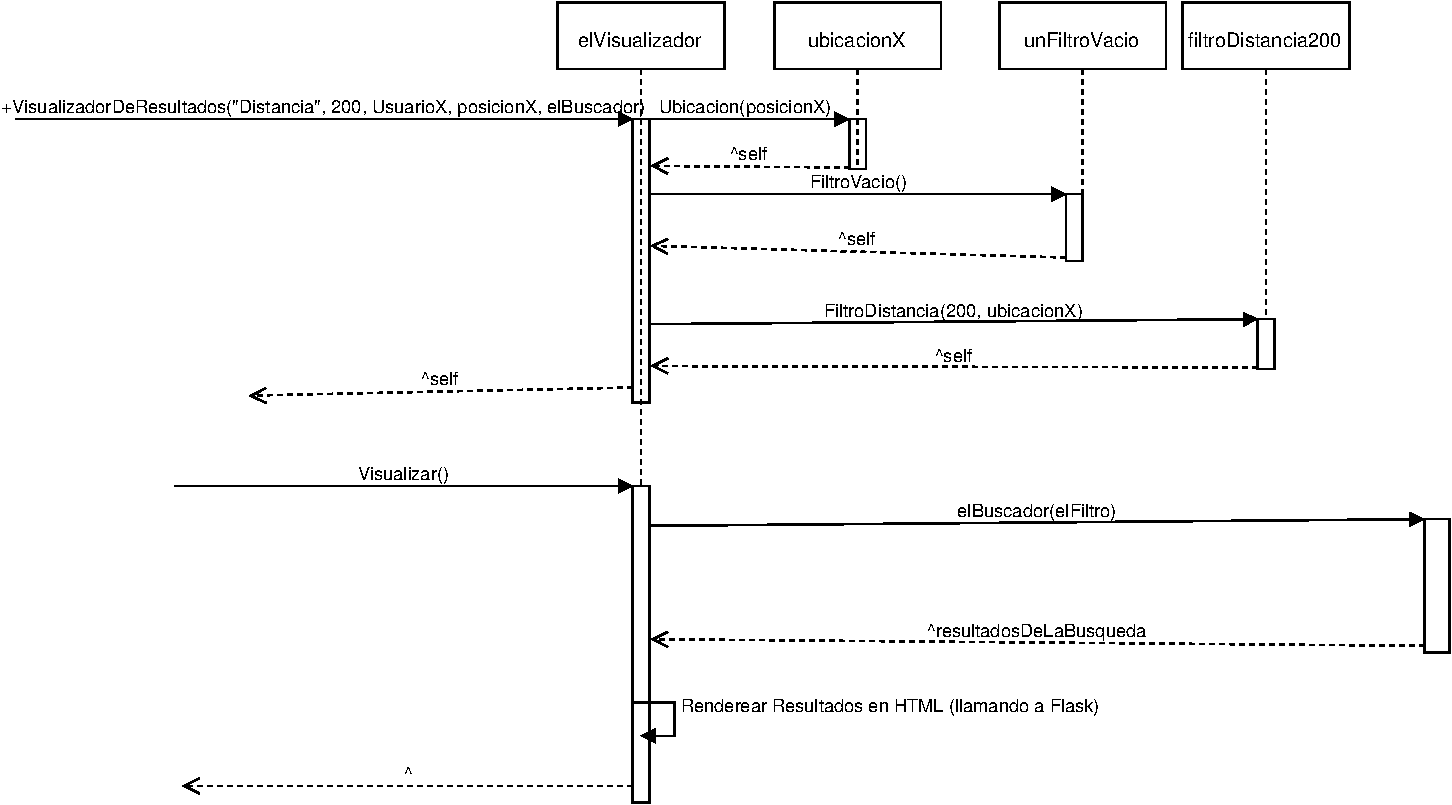
\includegraphics[width=\textwidth]{diagramas/secuencia_4.pdf}
  \caption{\normalfont Diagrama de secuencia.}
\end{figure}

\begin{figure}[H]
  \centering
  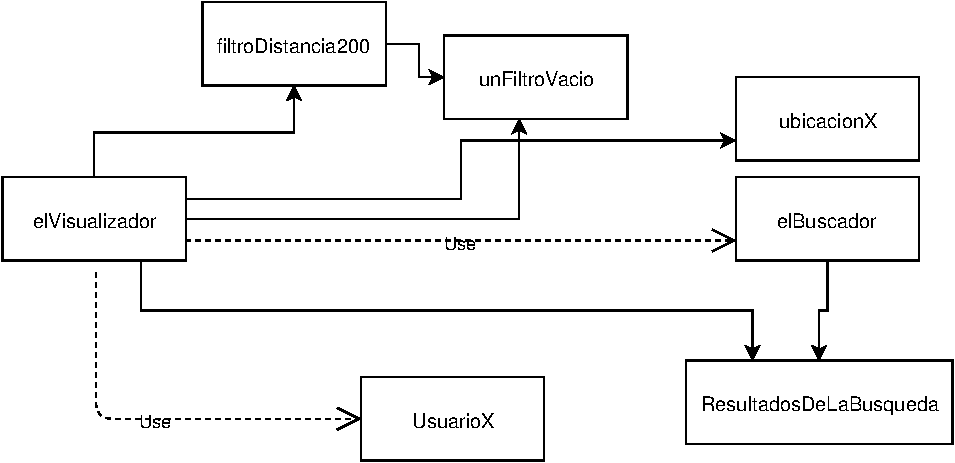
\includegraphics[width=0.7\textwidth]{diagramas/objetos_4.pdf}
  \caption{\normalfont Diagrama de objetos.}
\end{figure}

Como se ve, hay muchos objetos que interactúan. Esto no quiere decir que el acoplamiento sea alto, debido a que los objetos que interactúan tiene sentido que interactuen para mostrar los resultados.

\subsubsection{Autenticar Usuario}

\par A continuación presentamos los diagramas de objetos y secuencia de una llamada (exitosa) a 
\texttt{ElConjuntoDeUsuarios.autenticar(UnUsername, UnaPassword)} durante el proceso de \textit{log-in}.

\begin{figure}[ht]
    \centering
    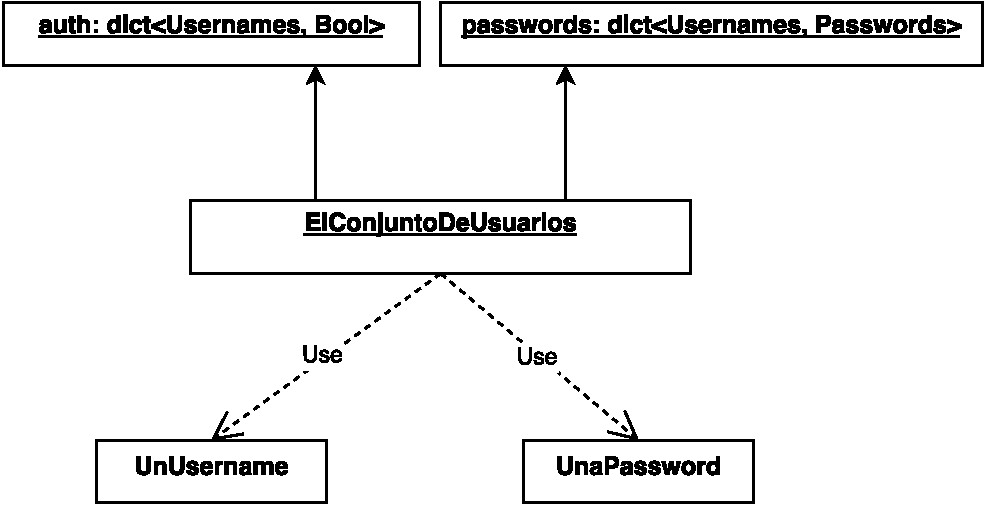
\includegraphics[width=0.9\textwidth]{diagramas/ObjetosLogIn.pdf}
    \caption{Diagrama de objetos de una autenticación (exitosa).}\label{ObjLogIn}
\end{figure}

\begin{figure}[ht]
    \centering
    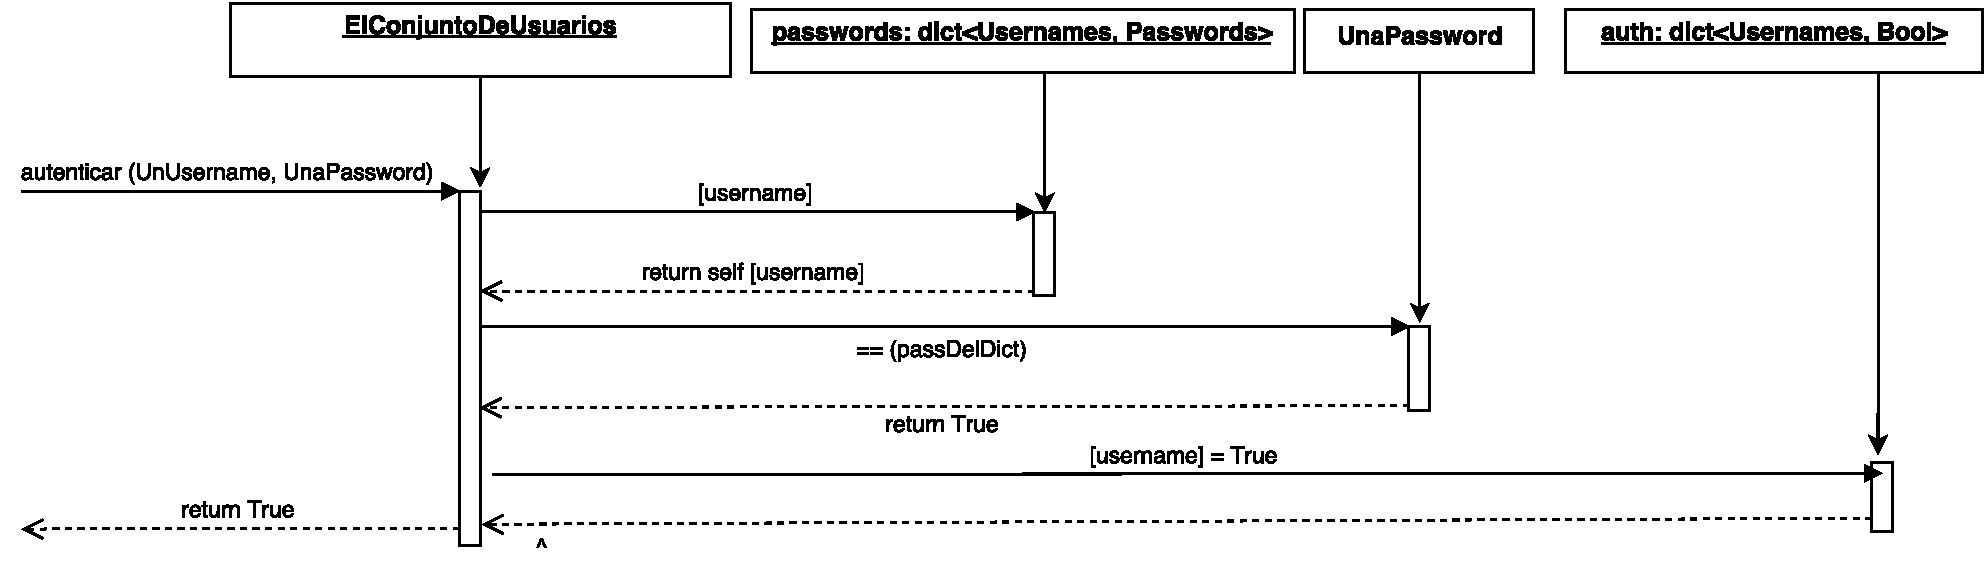
\includegraphics[width=0.9\textwidth]{diagramas/SecuenciaLogIn.pdf}
    \caption{Diagrama de secuencia de una autenticación (exitosa).}\label{SecLogIn}
\end{figure}

\par Si bien el proceso de \textit{log-in} es más extenso que la llamada a \texttt{autenticar}, lo omitido está relacionado a \textit{Flask}, rendering de html, llenado de \textit{forms} y demás; tales detalles son ortogonales al diseño planteado, por lo que sólo presentamos dicha llamada.

\par Se muestra un caso exitoso; si falla la búsqueda en el diccionario (al no existir el usuario) o la comparación entre \textit{passwords}, se levanta una excepción que la función de \textit{log-in} captura y reacciona correspondientemente.

\subsection{Más en detalle\ldots}

\subsubsection{Incorporación de bares}

\subsubsection{Incorporación de nuevas características de bares}

Como nosotros tomamos la decisión de diseño de que las features no sean ``positivas o negativas'', si no porcentuales, la feature que agregaríamos valoraría la calidad de los espectáculos, y en caso de que no haya, valdrá 0.

Agregar esto no sería nada difícil, sólo habría que agregar un campo mas a los features de la clase Valoración (además de cambiar los templates HTML para que muestren la nueva información).

En caso que se quisiera filtrar además por la feature de los espectáculos en vivo, se deberá agregar una nueva clase que herede de FiltrosExtra y filtre por esta categoría.

Como se ve, las modificiaciones involucran solo agregar código (y modificar Valoración, que es correcto que deba modificarse), con lo que el diseño es resiliente frente a este eje de cambio.

\subsubsection{El diseño y comportamiento de los distintos filtros de búsqueda de bares}

Recordemos cómo era el diagrama de clases de los filtros.

\begin{figure}[H]
  \centering
  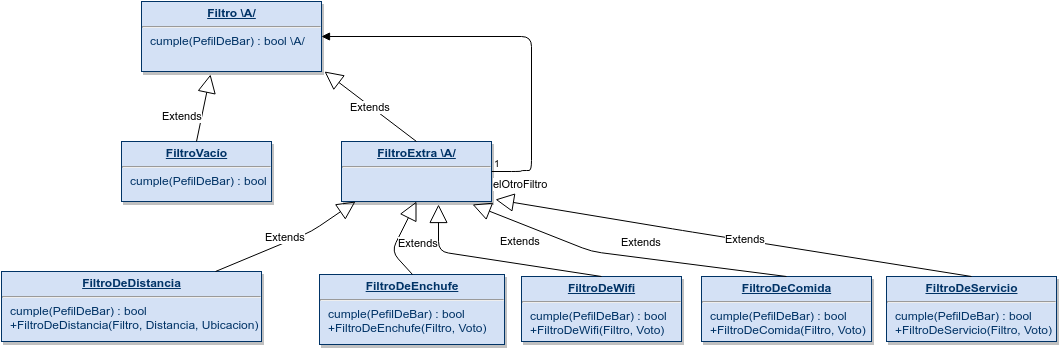
\includegraphics[width=\textwidth]{diagramas/filtro_clases.png}
  \caption{\normalfont Diagrama de clases.}
\end{figure}


Como dijimos anteriormente, los filtros los diseñamos usando el patrón Decorator.Elegimos este patrón porque parecía el más natural para resolver el problema y efectivamente lo era.

Recordemos que el ``intent'' del patrón Decorator es ``Asignar responsabilidades a un objeto dinamicamente y proveer una alternativa a la subclasificación para extender'', que es exactamente lo que queremos hacer aquí, queremos, dinámicamente, poder crear un filtro de distintas features dinámicamente.

En cuanto al funcionamiento, fue explicado intensamente en la sección anterior, con dos diagramas de objetos y dos diagramas de secuencia que dejan en claro como van a interactuar los objetos.

Luego de finalizar el diseño y la implementación, notamos que quizás todos las subclases de FiltroExtra (excepto FiltroDeDistancia), podrían contraerse a una única clase. 

Sin embargo, esto no formaba parte del sprint, con lo cual la refactorización de este código quedará para un sprint futuro. Además, los Product Owner indicaron que el diseño de filtro era el esperado, con lo cual quizás ni siquiera haya que cambiarlo.

Los filtros podrían ser contraídos a un FiltroDeFeature, que toma como parámetro el string de un feature, y le pide ese feature a las valoraciones del perfilDeBar pasado como parámetro, y las compara. Esto permitiría ahorrar repetición de código, quizas perdiendo expresividad, por eso no nos parece un cambio del todo positivo, pero nos pareció importante decir que tuvimos en cuenta que esto era una alternativa y decidimos no hacerla.


